% Preamble
\documentclass[12pt, twoside]{book}
\usepackage[utf8]{inputenc}
\usepackage{graphicx}
\usepackage{amsmath}
\usepackage{amsfonts}
\usepackage{nicematrix}

\usepackage{datetime}

\newdateformat{monthyeardate}{%
  \monthname[\THEMONTH], \THEYEAR}
  
\graphicspath{ {images/} }

\usepackage[a4paper,width=150mm,top=20mm,bottom=20mm,bindingoffset=6mm]{geometry}

\usepackage{fancyhdr}
\pagestyle{fancy}
\fancyhead{}
\fancyhead[RO,LE]{Computational Topics on the Solution of Integral Equations}
\fancyfoot{}
\fancyfoot[LE,RO]{\thepage}
\fancyfoot[LO,CE]{Chapter \thechapter}
\fancyfoot[CO,RE]{Srinath Kailasa}

\usepackage{titlesec}

\titleformat{\chapter}[display]
  {\normalfont\bfseries}{}{0pt}{\Huge}

\usepackage[backend=bibtex]{biblatex}
\addbibresource{references.bib}


\usepackage{lipsum}
\usepackage[toc]{glossaries}

\makeglossaries
\newglossaryentry{FMM}{
    name={FMM},
    description={
    Fast Multipole Method.
    }
}

\newglossaryentry{HPC}{
    name={HPC},
    description={
        High Performance Computing.
    }
}

\newglossaryentry{flops}{
    name={flops},
    description={
        Floating Point Operations per Second.
    }
}

\newglossaryentry{API}{
    name={API},
    description={
        Application Programming Interface - the software interface to a library.
    }
}


\newglossaryentry{CPU}{
    name={CPU},
    description={
        Central Processing Unit
    }
}

% Default fixed font does not support bold face
\DeclareFixedFont{\ttb}{T1}{txtt}{bx}{n}{12} % for bold
\DeclareFixedFont{\ttm}{T1}{txtt}{m}{n}{12}  % for normal

% Custom colors
\usepackage{color}
\definecolor{deepblue}{rgb}{0,0,0.5}
\definecolor{deepred}{rgb}{0.6,0,0}
\definecolor{deepgreen}{rgb}{0,0.5,0}

\usepackage{listings}

% Python style for highlighting
\newcommand\pythonstyle{\lstset{
language=Python,
basicstyle=\ttm,
otherkeywords={self},             % Add keywords here
keywordstyle=\ttb\color{deepblue},
emph={MyClass,__init__},          % Custom highlighting
emphstyle=\ttb\color{deepred},    % Custom highlighting style
stringstyle=\color{deepgreen},
frame=tb,                         % Any extra options here
showstringspaces=false            %
}}


% Python environment
\lstnewenvironment{python}[1][]
{
\pythonstyle
\lstset{#1}
}
{}

% Python for external files
\newcommand\pythonexternal[2][]{{
\pythonstyle
\lstinputlisting[#1]{#2}}}

% Python for inline
\newcommand\pythoninline[1]{{\pythonstyle\lstinline!#1!}}

\begin{document}


    \begin{titlepage}
    \begin{center}
        \vspace*{1cm}

        \Huge
        \textbf{Computational Topics on the Solution of Integral Equations}

        \Large
        \vspace{0.5cm}
        %Subtitle

        \vfill

        \textbf{Srinath Kailasa}

        \vspace{5cm}

        A thesis submitted in partial fulfillment of the requirements for the
        degree Doctor of Philosophy 

        \vspace{0.8cm}

        % 
\includegraphics[width=0.4\textwidth]{university.png}

        \large
        Department of Mathematics\\
        University College London\\
        \monthyeardate\today

    \end{center}
 \end{titlepage}

    \thispagestyle{plain}

\begin{center}
    \textbf{Declaration}
\end{center}
I, Srinath Kailasa, confirm that the work presented in this thesis is my own. Where information has been derived from other sources, I confirm that this has been indicated in the thesis.


\begin{center}
    \textbf{Acknowledgements}
\end{center}

The completion of this thesis simply wouldn't have been possible without the strong prevailing wind of emotional support from my family the regularity of fun with my friends, and the sympathetic and dedicated teachers and colleagues I met at UCL and across the world. Thank you \textit{all} for giving me this opportunity, I'm excited for what the future brings.

\begin{center}
   {\tel ఇది మా అమ్మ కోసం రాశాను}
\end{center}

    \newpage

    \thispagestyle{plain}

\begin{center}
    \textbf{Abstract}
\end{center}

Integral equation methods are a powerful technique for the solution of the boundary value problems that arise from electromagnetic and acoustic scattering. This is due to the fact that they reduce problems defined over unbounded domains into ones defined by a boundary integral. The principle drawback of such methods is the dense linear matrix that must be either applied or inverted in the resulting linear system upon discretisation, depending on whether one is solving the forward or inverse problem. The past three decades have seen the development of techniques that allow for the

This thesis is concerned with the development of simulation methods and software for the rapid forward and inverse applications of the discrete operators arising in boundary integral formulations of scattering problems, the overarching goal being fully parallelised simulation software for the

    \tableofcontents

    \chapter{Modern Programming Environments for Science}\label{chpt:1:modern_programming_environments_for_science}
- Brief motivation behind fast particle solvers, and where they fit in the scientific landscape, why are they useful?

- Brief survey on other uses of FMM (Kalman filtering - covariance matrices), lead into application for integral equations which is our motivating application

- Give a sense of the scale of improvement that these methods provide for solving this class of problems - making integral equations practicable computational techniques is a big deal.

~ 1 page 
\section{Pitfalls of Performant High Level Language Runtimes}\label{chpt:1:sec:1}

The evolution of computational science has been marked by the introduction and adoption of high-level interpreted languages that are designed to be user friendly, and cross platform. Starting with Matlab in the 1970s, followed by Python in the 1990s, and more recently Julia in the 2010s. High-level languages have significantly impacted scientific computing, offering efficient implementations of algorithms and introducing optimised data structures via projects such as NumPy and SciPy, as well as ergonomic cross platform build systems. While these languages facilitate easier experimentation, achieving peak performance often necessitates manual memory management or explicit instruction set level programming to ensure vectorisation on a given hardware target. A natural question for us when deciding on a programming environment for this project was whether advancements in high-level languages were sufficient for the implementation of `fast algorithms'. If they proved to be sufficient our software would be free of the so called `two language' problem, in which a user friendly interfaces in a high-level language provides a front-end for a compiled language implementation of more data-intensive operations. This problem plagues academic software development, as resulting software relies on a brittle low-level interface between the high-level front-end, and low-level back-ends for performance critical code sections.

Recent strategies to enhance the performance of high-level languages have involved refining compiler technology. These projects are advertised as tools that allow developers to use high-level languages for quick algorithm experimentation, while leaving it to the compiler to produce efficient machine code. Benchmarks are usually offered with respect certain numerical operations that can be vectorized, such as iteration over aligned data structures, with compilers taking care to unroll loops and apply inlining to inner function calls.

Noteworthy examples are the Numba project for Python and the Julia language. Both leverage the LLVM compiler infrastructure, which aims to standardize the back-end generation of machine code across various platforms. This approach, known as 'just in time' or JIT compilation, generates code at runtime from the types of a function's signature. Figure \ref{fig:chpt:1:sec:1:numba_runtime} provides a sketch of how Numba in particular generates machine code from high-level Python code. The LLVM compiler supports numerous hardware and software targets, including platforms like Intel and Arm, and provides multithreading through support for compiler extensions such as OpenMP. Additionally, these compilers offer native support for GPU code generation. An important difference between Numba and Julia is that Numba is simply a compiler built to optimise code written for the numerical types created using the NumPy library, and Julia is a fully fledged language. Numba contains implementations of algorithms a subset of the scientific Python ecosystem, specifically functionality from the NumPy project for array manipulation and linear algebra.

% Many `fast algorithms', such as the Fast Multipole Method (FMM), depend on hierarchical data structures. For instance a `quadtree', in two dimensions, and an `octree', in three dimensions. Here, each tree node points to either four or eight child nodes, respectively. A natural implementation makes use of pointers linking blocks of memory holding node data \cite{sundar2008bottom}. However, this method presents challenges in high-level programming environments that don't expose memory management to developers, and we are forced to linearise the data structure by making use of a linear blocks of memory to store node information, and vectors of index pointers to look up data.

As many performance benchmarks for these programming environments are typically provided for algorithms that rely on simpler data structures, we decided to test these high-level environments for more complex algorithms before making a choice about our programming environment for this project. We implemented a single node multi-threaded FMM using Python's Numba compiler, identifying two notable pitfalls with this approach, the full results of which were recently published in Computing in Science and Engineering \cite{kailasa2022pyexafmm}.

Firstly, JIT compilation of code imposes a significant runtime cost that is disruptive to development. Compiled functions are by default not cached between interpreter sessions in either Julia or Numba code. Our FMM code takes $15 \pm 1$s to compile when targeting a i7-9750H CPU with x86 architecture, where the benchmark is given with respect to seven runs. This is comparable to the runtime of the FMM software for a typical benchmark FMM problem \footnote{1e6 particles distributed randomly, using order $p=6$ expansions for a Laplace problem takes approximately 30s on this hardware using our software. See Chapter \ref{chpt:2:designing_software_for_fast_algorithms} for more details on the FMM and the significance of these terms.}. For smaller problem sizes, the compilation time dominates runtime. Ahead of time (AOT) compilation is partially supported in Numba, and can be used to build binaries for distribution to different hardware targets, e.g. x86 or ARM. However support for AOT compiled code is currently second class, the machine code created in this manner are usable only from the Python interpreter and not from within calls made from other Numba compiled functions, and it's currently staged for deprecation and replacement. We note that Julia does support AOT compilation via the PackageCompiler.jl module. This allows for different levels of AOT compilation, from creating a `sysimage' which amounts to a serialised file containing the compiled outputs of a Julia session, a relocatable `app' which includes an executable compiled to a specific hardware target alongside Julia itself, to creating a C library which can be precompiled for a specific hardware target such as x86. However, this requires relatively advanced software engineering skills, and raises the barrier to entry for high-performance computing with Julia.

Thus switching to such a programming environment requires developers to create a workflow that keeps interpreter sessions active for as long as possible in order to reduce the impact of long compilation times, or write build scripts for AOT compilation for a specific hardware target similar to compiled languages. As one of the key advantages of high-level languages is their developer friendliness and simple build systems this acts as an impediment.

Downstream users of software, who may also be using JIT compilers for their own code, are faced with significant compilation times, and potentially intricate build steps unless catered for by the original library's developers. This problem compounds in the case of distributed memory programs using MPI, as JIT compilation imposes runtime costs to the entire program. Unless a project has been distributed as a binary, by default MPI runs are not interactive, and therefore require a recompilation for each run. This isn't to say MPI programs written in Julia or Numba haven't been scaled to large HPC systems, however their usage does carry a cost in terms of developer workflow, and potentially program runtime, which can be significant if one is trying to reach the highest levels of performance.

Secondly, our experience in developing the FMM in Numba made clear how difficult it can be to anticipate the behaviour of Numba when considering how to optimise functions with different implementations of the same logic. Consider the code in Listing \ref{code:chpt:1:sec:1:numba_compiler_optimisations}, here we show three logically equivalent ways of performing two matrix-matrix products, and storing a column from the result in a dictionary. A dictionary is chosen for storage as this mirrors the data structure used in our FMM software for storing intermediate results. The runtimes of all three implementations are shown in Table \ref{table:chpt:1:sec:1:numba_compiler_optimisations} for different problem sizes. We choose this example because this operation of matrix-matrix multiplication is well supported by Numba, and data instantiation, whether from within or external to a Numba compiled function, should in principle make little difference as the Numba runtime simply dereferences pointers to heap allocated memory when entering a Numba compiled code segment. This example is designed to illustrate how arbitrary changes to writing style can impact the behavior of Numba code. The behavior is likely due to the initialisation of a dictionary from within a calling Numba function, rather than an external dictionary, and having to return this to the user. However, the optimisations taken by Numba are presented opaquely to a user and it's unclear why there are performance variations at all.

In developing our FMM code we faced significant challenges in tweaking our code and data structures to maximise the performance achieved from within Numba. From manually inlining subroutines as in Listing \ref{code:chpt:1:sec:1:numba_compiler_optimisations}, to testing where to allocate data. Our final code took a significant amount of time to develop, approximately six months, and was organised in a manner that optimised for performance rather than readability. Thus, despite being a \textit{compiler} for numerical Python, Numba behaved in practice more like a \textit{programming framework} which a developer had to adhere to strictly in order to achieve the highest-level of performance. The disadvantage of this is that the framework is both relatively restrictive, but also presented opaquely to a user.

Therefore, while being an amazing technology with great features, Numba was not decided to be a suitable choice for our programming environment. Its ability to target a diverse set of hardware targets from Python, leveraging the power of LLVM to write multithreaded, and autovectorised code, as well as writing CPU and GPU code from within Python, while allowing downstream projects to develop in a familiar language with a large open-source ecosystem and simple dependency management demonstrate the utility of this remarkable tool. However, the constraints of high level languages, specifically the inability to manage memory at a system level, as well as the development costs of JIT compilation, and Numba's framework-like behaviour demonstrate that while being useful, it is preferable to write our software platform using a systems-level language where high-performance can be assumed. Our criticisms of Numba also apply to Julia. However we note that Julia has certain advantages over Numba including its design and syntax focussed on mathematical computing, native support for multithreading, a richer type system and a large open-source community with a scientific computing focus.

System level languages have progressed commensurately to high-level languages over recent decades. Modern languages such as Go and Rust, offer runtimes with informative compilers, inbuilt documentation and testing facilities, as well as LLVM backends to support code generation across platforms, removing much of the complexity associated with building and distributing software written in C/C++. Rust in particular, uninhibited by a garbage collector as for Go, makes it easy to interoperate Rust code with libraries built in C/C++ via its foreign function interface, making it simple to leverage existing open-source scientific software.  We therefore conclude that the two language problem is minimised in comparison to the past, and modern system level programming languages potentially offer an effective solution for building academic software.

\begin{figure}[h]
    \centering
    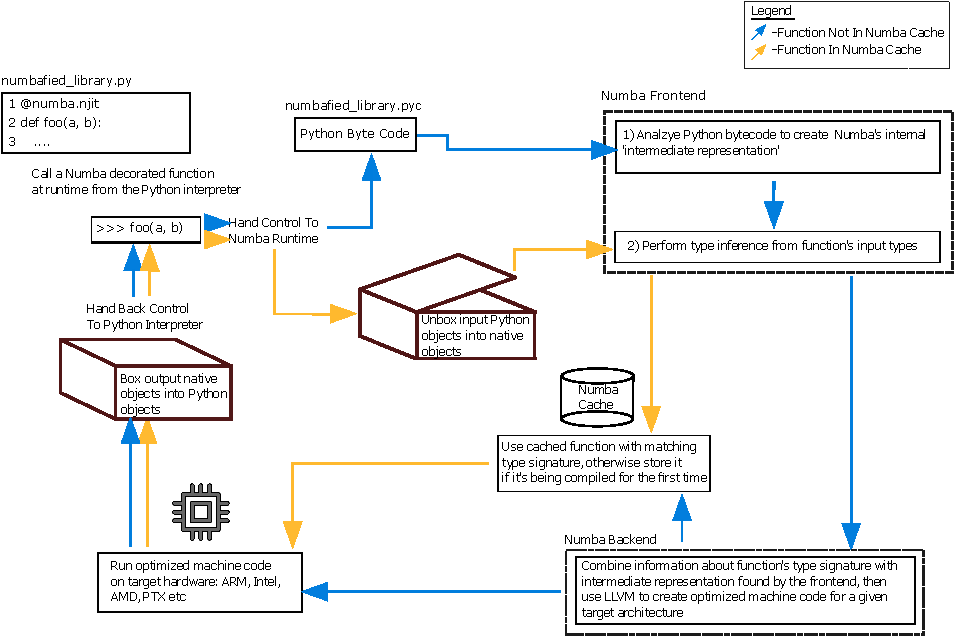
\includegraphics[width=\linewidth]{images/ch_1/numba.pdf}
    \caption{A visualisation of the Numba runtime system. A function decorated with `njit' acts as an instruction to the runtime to check a database for any Numba-compiled functions with a matching function signature, if this doesn't exist Numba generates a new compiled function and caches it using LLVM. Future calls of this function use this cached version in place of the Python interpreter. Code relies on Numba's runtime to correctly `box' and `unbox' native Python objects into data structures compatible with Numba code, which operates on a subset of numerical data structures created using the NumPy library. Figure adapted from \cite{kailasa2022pyexafmm}.}
    \label{fig:chpt:1:sec:1:numba_runtime}
\end{figure}


\pagebreak

% \begin{figure}[H]
\begin{lstlisting}[language=Python, caption={Three ways of writing a trivial algorithm in Numba, that performs some computation and saves the results to a dictionary. Adapted from Listing 2 in \cite{kailasa2022pyexafmm}},  label=code:chpt:1:sec:1:numba_compiler_optimisations]
import numpy as np
import numba
import numba.core
import numba.typed

# Initialise in the Python interpreter
data = numba.typed.Dict.empty(
    key_type=numba.core.types.unicode_type,
    value_type=numba.core.types.float64[:]
)

data['initial'] = np.ones(N)

# Subroutine 1
@numba.njit
def step_1(data):
    """
    Initialise a matrix and perform a matrix matrix product,
    storing a single column in the data dictionary.
    """
    a = np.random.rand(N, N)
    data['a'] = (a @ a)[0,:]


# Subroutine 2
@numba.njit
def step_2(data):
    """
    Initialise a matrix and perform a matrix matrix product,
    storing a single column in the data dictionary.
    """
    b = np.random.rand(N, N)
    data['b'] = (b @ b)[0,:]


@numba.njit
def algorithm_1(data):
    """
    First implementation.
    """
    step_1(data)
    step_2(data)


@numba.njit
def algorithm_2(data):
    """
    Second implementation.
    """
    # This time the storage dictionary is created within the
    # Numba function, so the types are inferred by the Numba
    # runtime, this also avoids a boxing cost to create a Numba
    # type from a Python one.
    data = dict()
    data['initial'] = np.ones(N)
    step_1(data)
    step_2(data)
    return data

@numba.njit
def algorithm_3(data):
    """
    Third implementation.
    """

    # This time, the subroutines are manually inlined
    # by the implementer, as well as the initialisation
    # of the results dictionary locally, as in algorithm_2.

    data = dict()
    data['initial'] = np.ones(N)

    def step_1(data):
        a = np.random.rand(N, N)
        data['a'] = (a @ a)[0,:]


    # Subroutine 2
    @numba.njit
    def step_2(data):
        b = np.random.rand(N, N)
        data['b'] = (b @ b)[0,:]

    step_1(data)
    step_2(data)
    return data
\end{lstlisting}
% \end{figure}
% \afterpage{\clearpage}


\begin{table}
    \centering
    \caption{Performance of different algorithms from Listing \ref{code:chpt:1:sec:1:numba_compiler_optimisations}, taken on an i7 CPU and averaged over seven runs for statistics.}
    \begin{tabular}{l l l}
        \toprule
        Algorithm & Matrix dimension & Time ($\mu s$) \\
        \midrule
        1 & \(\mathbb{R}^{1 \times 1}\) & 1.55 $\pm$ 0.01 \\
        1 & \(\mathbb{R}^{100 \times 100}\) & $304 \pm 3$\\
        1 & \(\mathbb{R}^{1000 \times 1000}\) & $29,100 \pm 234$ \\
        \midrule
        1 & \(\mathbb{R}^{1 \times 1}\) & $2.73 \pm 0.01$ \\
        1 & \(\mathbb{R}^{100 \times 100}\) & $312 \pm 3$ \\
        1 & \(\mathbb{R}^{1000 \times 1000}\) & $25,700 \pm 92$ \\
        \midrule
        1 & \(\mathbb{R}^{1 \times 1}\) & $2.71 \pm 0.01$ \\
        1 & \(\mathbb{R}^{100 \times 100}\) & $312 \pm 1$ \\
        1 & \(\mathbb{R}^{1000 \times 1000}\) & $25,700 \pm 140$ \\
        \bottomrule
    \end{tabular}
    \label{table:chpt:1:sec:1:numba_compiler_optimisations}
\end{table}

\section{Introducing Rust for Scientific Software}\label{chpt:1:sec:2}

Rust is a modern system-level programming language, introduced by Mozilla in 2015 as a direct replacement for C/C++, and is bundled with features that favour safety for shared memory programming. Having identified it as a suitable candidate for our programming environment, we list a few of its key benefits in this section.

Fortran and C/C++ have have continued to dominate high-performance scientific computing applications, the main criticism of these languages for academic software is their relatively poor developer experience. C/C++ especially has significant flexibility in the compilers, documentation, build systems and package managers that developers can choose to work with, as well as support for multiple paradigms and a growing syntax. Rust stands in contrast to this with a single centrally supported runtime system, Cargo, with common standards for testing and documentation. Additionally, there is only a single Rust compiler, rustc. This inflexibility, in addition to a strongly preferred way of organising Rust code via its Traits system, makes Rust libraries significantly more uniform and readable than corresponding C++ code. Indeed installing a Rust library, or building a binary, is often as simple as running a single command from a terminal, or adding a single line to a TOML dependency file.

The lack of a uniform building and packaging standards in C/C++ means that some projects go as far as to implement a custom build system, such as the Boost library \cite{boostbuild2022github}. With the exception of Fortran, which has made recent strides to develop a standardised modern package manager and build system, inspired by Rust's Cargo \cite{fpm2022github}, C and C++ do not have a single officially supported package manager or build system. The resulting landscape is a multitude of package managers \cite{spack2022github, vcpkg2022github, conan2022github} and build systems \cite{meson2022github, bazel2022github, scons2022github} a few of which we have cited here, all of which replicate each others functionality, none of which are universally accepted or implemented across projects nor officially supported by the C++ software foundation. Figure (\ref{fig:chpt:1:sec:2:builds}) provides an overview of a few of the myriad approaches taken in other languages. To manage this complexity, builds are often defined using a metabuild system, most commonly CMake. CMake is a scripting language, and as a meta build system it takes a specification of local and third party dependencies and hardware targets, and generates Makefiles. CMake gives developers a great deal of flexibility, it is multi-platform, and language agnostic, however it is not straightforward to maintain projects as the number of dependencies grows. Indeed, there is a significant body of literature discussing best practices with CMake \cite{scott2018professional}. However, CMake is not responsible for downloading and installing third party packages or verifying their relative compatibility, implementing its best practices is again left to users. Cargo's relative simplicity mirrors the simple build systems of high-level languages such as Python or Julia, and removes one of the main causes of development pain when working with compiled languages, and makes it significantly easier for small teams to publish software that can be easily deployed by downstream users regardless of their system's architecture or operating system.

A unique feature of Rust is its approach to ensure safe shared memory programming, enforced by its compile time `borrow checker'. Every reference in Rust has an associated `lifetime' defined by its scope, and a singular `owner'. Which enforce the programming pattern of `resource allocation is initialisation' (RAII). The basic rule is that references are owned within a scope, and dropped when out of scope. The borrow checker enforces this at compile-time, in a multithreaded context this makes it impossible to have a compiled Rust binary that has dangling pointers or double-free errors. For mutable data, the borrow checker ensures that there is only a single mutable reference at any given time in the program's runtime, ensuring that there can never be a race condition in compiled Rust code. Identifying pointer-related bugs is one of the main challenges in multi-threaded programming, with safe `smart pointers' being optional in C++, implementing RAII is left to developers.

Rust is `multi-paradigm', supporting both object oriented, and functional styles of programming. Method calls are often chained, in a functional-like style, however users can still implement methods on structs as in other object oriented languages. The unique feature introduced by Rust is its Traits system, for specifying shared behaviour, that supersedes object-oriented design. Traits are a similar to C++ 20's interfaces, in that they provide a way to enforce behaviour, rather than embedding it into a type as with traditional inheritance. However unlike C++, Rust Traits allow you to write blanket implementations, and implement interfaces for types you didn't define in your own code making them significantly more powerful. This means that behaviour can be built `bottom up', rather than `top down' as with object orientation, making it much easier for readers to identify the expected behaviour of a given Rust type by simply reading which Traits it implements. In a scientific context we are usually concerned with the organisation, reading and writing of data, commonly adhering to a design philosophy known to as data-oriented design. Traits allow us to inject additional behaviour on types without having to worry about potentially complex inheritance hierarchies.

Rust's runtime includes a test runner, a documentation generator, and a code formatter. As with other Rust features, these are maintained in lock step with the language specification, and with reference to other Rust developments. This imposes universal constraints on all Rust projects, allowing for objectively defined `good' Rust code, rather than relying on various standards of best practices that vary between projects and organisations. Furthermore the Rust compiler is highly informative, providing hints to developers on best practices for their code, as well as potential sources of bugs or code rot, by notifying users of common anti-patterns or unused variables and functions.

Despite being a young language, Rust already supports a mature ecosystem of libraries for scientific computing with high-level multithreading support \cite{rayon2018github}, numerical data containers \cite{ndarray2022github}, and tools for generating interfaces to Python via its C ABI \cite{maturin2022github}. Many tools are yet to be ported into native Rust, however high quality bindings exist for core tools such as MPI \cite{rsmpi2018github}, BLAS and LAPACK \cite{blaslapackrust2022github}, with simplified build steps often requiring only a few extra lines in the dependency TOML file. The problem with interfacing with tools written in other languages is also present when building software in Rust, however Cargo offers tools to build software written in other languages and integrate it with Rust code via the `build.rs' package, which allows one to leverage existing build systems written for software written in foreign languages. This detracts from the benefits offered by Cargo as a unified package manager and build system, raising similar problems to those encountered when building software in other compiled languages. However, we observe that this remains a concern of the software's developer, who is responsible for providing build scripts for the operating systems and hardware platforms that they wish to support, and from a downstream user perspective their build process remains the same as with pure Rust packages, where the dependency is defined in their dependency TOML file. We also note that Rust is missing key tools for scientific computing, such as a code generation for GPUs, however with mounting interest in Rust from the scientific computing community this is an active area of development.


\begin{figure}
    \centerline{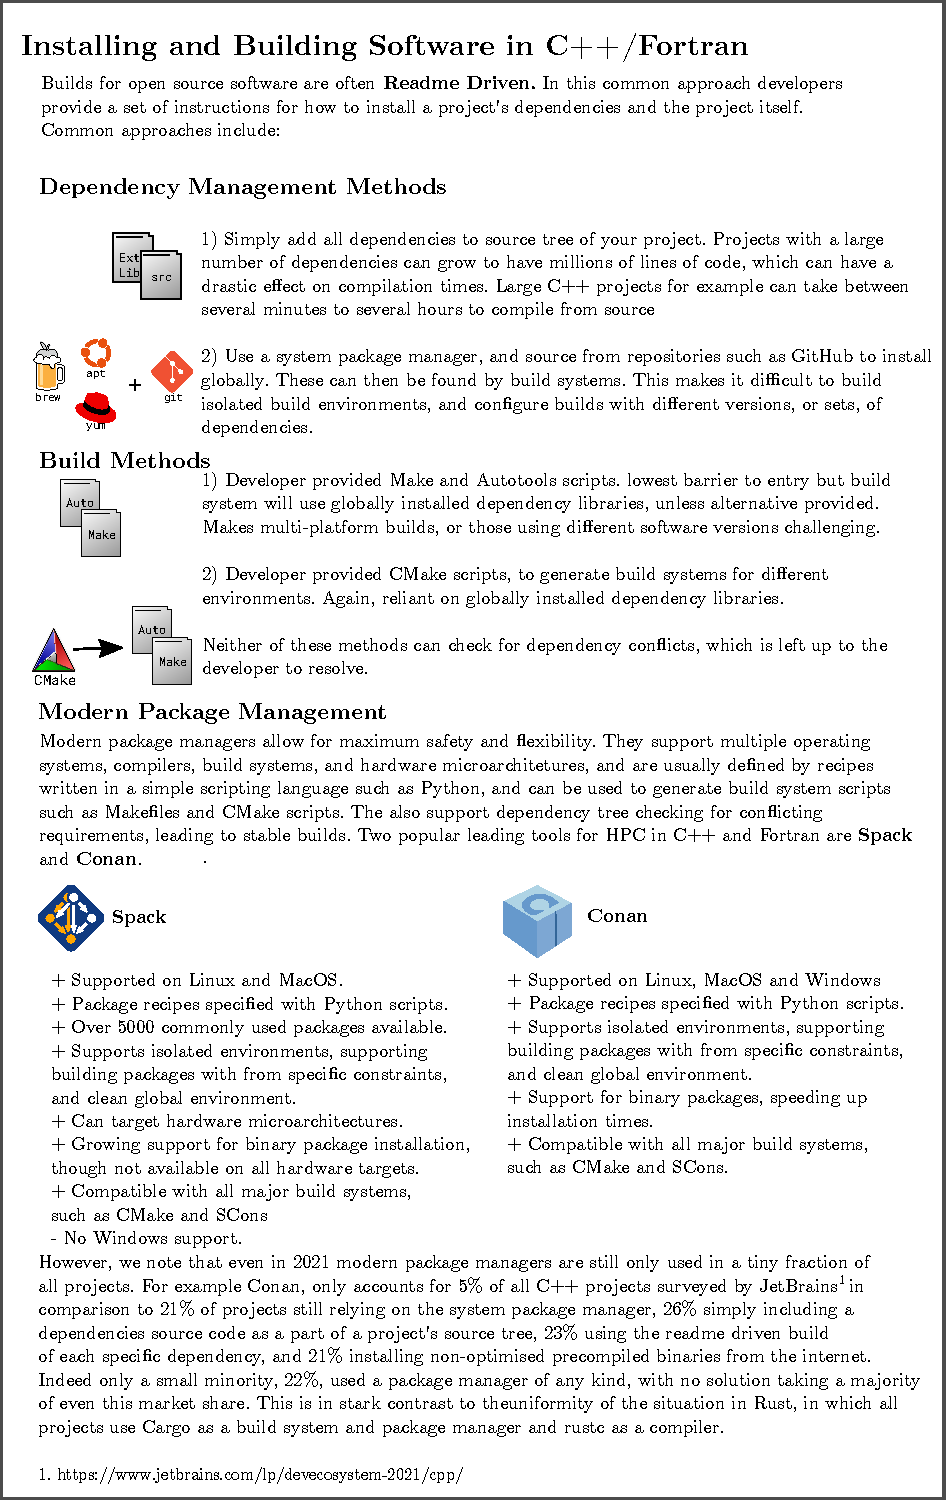
\includegraphics[width=0.95\linewidth]{ch_1/builds.pdf}}
    \caption{An overview of building software in other compiled languages.}
    \label{fig:chpt:1:sec:2:builds}
\end{figure}

\section{Future Developments}\label{chpt:1:sec:3}

Despite the above criticisms, high-level languages as tools for high-performance scientific computing remain an intense area of research and development. 'Mojo' is a new programming language, along with a compiler. It's built as a superset of Python, specifically with the two-language problem in mind. Additionally, it attempts to address the 'three language problem', whereby languages also target exotic hardware such as GPUs and TPUs \cite{Lattner2023Mojo}.

Led by a team that includes the original developers of LLVM, Mojo aims to simplify the development of high-performance applications in a Python-like language, that acts as a superset of Python. Moreover, it seeks to make these applications deployable across most hardware and software targets, ensuring compatibility with Python's vast open-source libraries and straightforward build tools.

This is achieved by building on the MLIR compiler infrastructure. MLIR can be thought of as a generalisation of LLVM, catering to CPUs, GPUs, and novel ASICs for AI. The team chose to develop around Python to leverage its extensive existing user base in computational and data sciences.

Currently, Mojo remains a closed-source language and is actively being developed by its parent company, Modular. Thus, even though it appears promising, it's not yet in a state suitable for experimentation. Nevertheless, Mojo showcases the potential of a future programming environment that might definitively `solve' the problems developers face when selecting a programming environment for academic software.

    \appendix
    \chapter{Appendix}

\section{Fast Multipole Method Algorithm}\label{app:a_1_fmm_algorithm}

FMM Algorithm logic as pseudocode.


    \printglossary

    \printbibliography[heading=bibintoc]


\end{document}